\section{Methods}

\begin{frame}
	\frametitle{1. Data Reduction}
	\framesubtitle{Problem: Too much data}
	\begin{figure}
	    \centering
	    \scalebox{0.4}{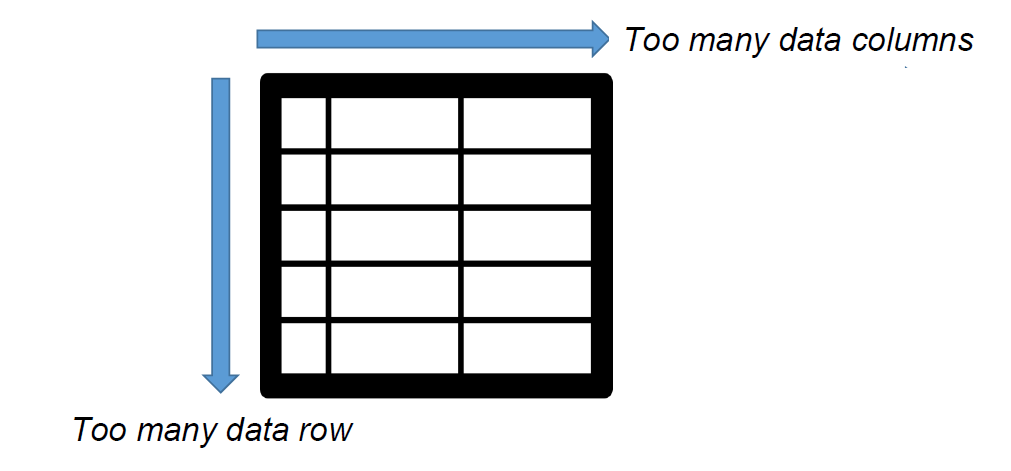
\includegraphics{figures/Problem_Data_Size}}
	    \caption{The challenge of large data is the \textit{vertical} and \textit{horizontal} data size}
	    \label{fig:toolarge}
	\end{figure}
\end{frame}

\begin{frame}
	\frametitle{1. Data Reduction}
	\begin{itemize}
		\item Vertical Data Reduction: \textit{Remove data rows}
		\begin{itemize}
		    \item Sampling
		    \item Filtering
		    \item Abstraction
		    \item Aggregation
		    \item ...
		\end{itemize}
		\item Horizontal Data Reduction: \textit{Reduce dimensions}
		\begin{itemize}
		    \item Projection
		    \item PCA, SOM
		    \item ...
		\end{itemize}
	\end{itemize}
\end{frame}

%%%%%%%%%%%%%%%%%%% Visualization %%%%%%%%%%%%%%%%%
\begin{frame}
	\frametitle{2. Scalable Visualizations}
	\begin{itemize}
		\item Techniques for large scale visualization
		\begin{itemize}
		    \item pixel-oriented techniques
		    \item projection techniques
		    \item hierarchical techniques
		    \item icon-based
		    \item (graph-based) 
		\end{itemize}
		\item Advanced Metaphors
		\begin{itemize}
		    \item Multi-Resolution
		    \item Aggregation-Markers
		\end{itemize}
	\end{itemize}
\end{frame}

\begin{frame}{2. Scalable Visualizations}
\begin{figure}
    \begin{subfigure}
        \centering
        \scalebox{0.2}{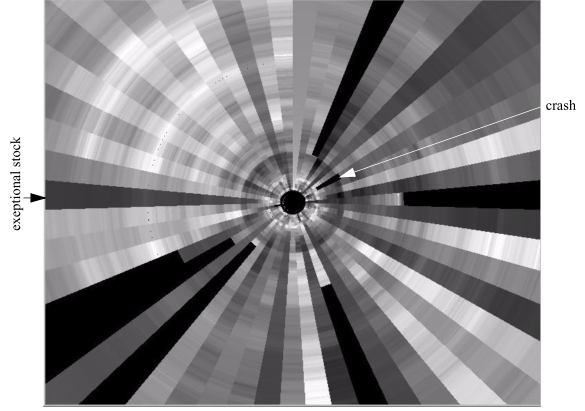
\includegraphics{figures/DataTube}}
        \caption{Pixel-Oriented Techniques}
        \label{fig:pixel-oriented}
    \end{subfigure}
    \begin{subfigure}
        \centering
        \scalebox{0.3}{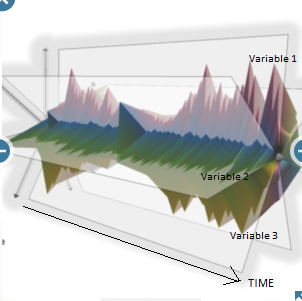
\includegraphics{figures/Kiviat}}
        \caption{Projective-Geometric Techniques}
        \label{fig:projective-geometric}
    \end{subfigure}
    
\end{figure}
\end{frame}

\begin{frame}{2. Scalable Visualizations}
\begin{figure}
    \centering
    \scalebox{0.5}{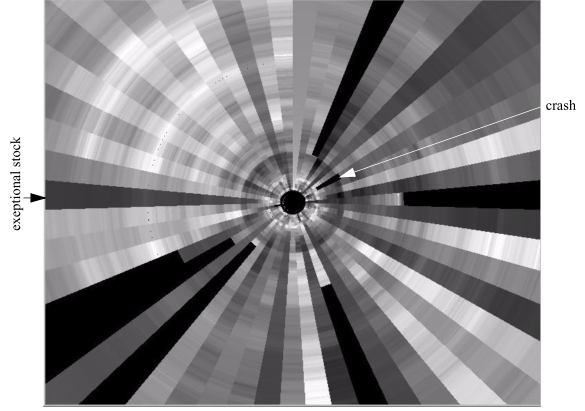
\includegraphics{figures/DataTube}}
    \caption{Pixel-Oriented Techniques}
    \label{fig:pixel-oriented-large}
\end{figure}
\end{frame}

\begin{frame}{2. Advanced Visual Metaphors}
    \begin{figure}
        \centering
        \scalebox{0.5}{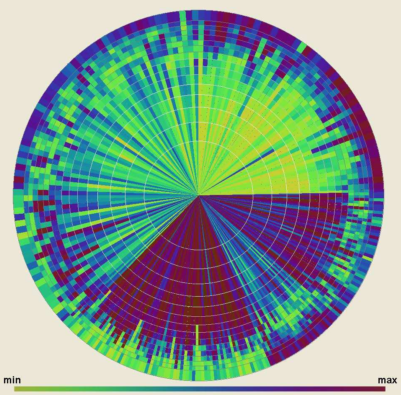
\includegraphics{figures/multi-resolution}}
        \caption{Multi-Resolution CircleView}
        \label{fig:multi-resolution}
    \end{figure}
\end{frame}

\begin{frame}{2. Advanced Visual Metaphors}
    \begin{figure}
        \centering
        \scalebox{0.5}{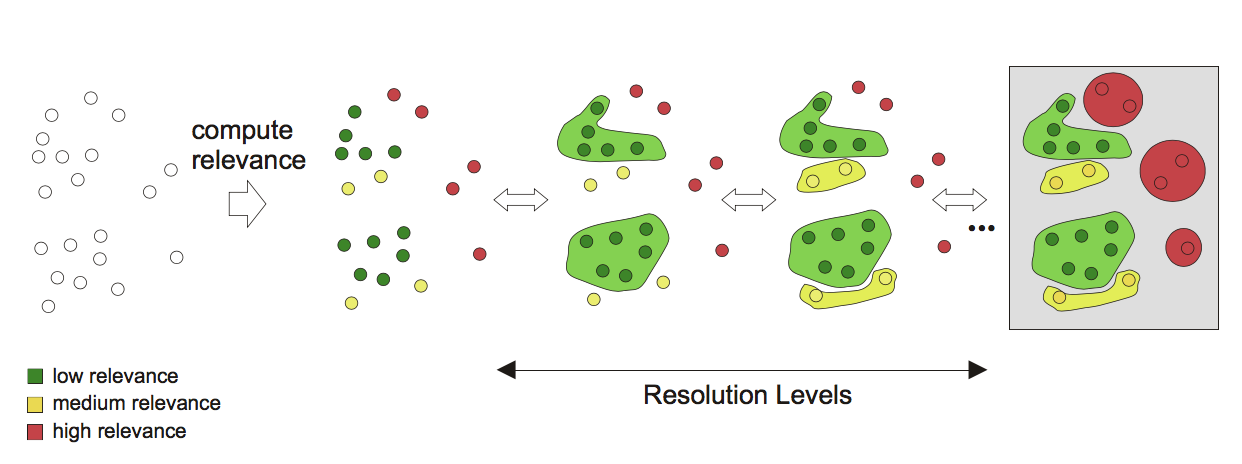
\includegraphics{figures/multi-resolution_explained}}
        \caption{Multi-Resolution}
        \label{fig:multi-resolution-explained}
    \end{figure}
\end{frame}

\begin{frame}{2. Advanced Visual Metaphors}
\begin{itemize}
    \item \href{http://bl.ocks.org/gisminister/10001728}{Marker Clustering}
    \item \textit{Smart Data Compression}
\end{itemize}
\end{frame}

\begin{frame}
	\frametitle{3. Interaction}
	\begin{itemize}
		\item Standard Techniques
		\begin{itemize}
		    \item Zoom
		    \item Filter
		\end{itemize}
		\item Distortion Techniques
		\begin{itemize}
		    \item \href{https://bost.ocks.org/mike/fisheye/}{\textit{Fish-Eye}}
		    \item Perspective Wall
		\end{itemize}
		\item Navigation Techniques
		\begin{itemize}
		    \item Navigational Maps
		    \item Search
		    \item Coordinated Windows
		\end{itemize}
	\end{itemize}
\end{frame}